\documentclass[oneside,bachelor,etd]{BYUPhys}
\usepackage{ifpdf}
\ifpdf
  \usepackage[pdftex]{graphicx}
\else
  \usepackage[dvips]{graphicx}
\fi

\usepackage{fancyhdr}
  \fancyhead{}
  \fancyhead[LO]{\slshape \rightmark}
  \fancyhead[RO,LE]{\textbf{\thepage}}
  \fancyhead[RE]{\slshape \leftmark}
  \fancyfoot{}
  \pagestyle{fancy}
  \renewcommand{\chaptermark}[1]{\markboth{\chaptername \ \thechapter \ \ #1}{}}
  \renewcommand{\sectionmark}[1]{\markright{\thesection \ \ #1}}

\usepackage[margin=0.3in,labelfont=bf,labelsep=none]{caption}
 \DeclareCaptionFormat{suggested}{\singlespace#1#2 #3\par\doublespace}
 \captionsetup{format=suggested}

\usepackage{cite}

\usepackage{makeidx}
\makeindex

\usepackage{url}
\urlstyle{rm}

\usepackage[bookmarksnumbered,pdfpagelabels=true,plainpages=false,colorlinks=true,
            linkcolor=black,citecolor=black,urlcolor=blue]{hyperref}

\usepackage{float}
\usepackage{color}
\usepackage{xcolor}
\usepackage{listings}
\usepackage{caption}

\DeclareCaptionFont{white}{\color{white}}
\DeclareCaptionFormat{listing}{\colorbox{gray}{\parbox{\textwidth}{#1#2 #3}}}
\captionsetup[lstlisting]{format=listing,labelfont=white,textfont=white}

% ------------------------- Fill in these fields for the preliminary pages ----------------------------
  \Year{2011}
  \Month{January}
  \Author{Oliver Lorenz}
  \TitleTop{SCd}
  \TitleBottom{Section Control Daemon}

  \Abstract{

Kapsch TrafficCom invented a new technique to increase data privacy on Section Control systems 
because current laws state that operating aforesaid systems infringes \S 1 of Austria's Data Privacy Law (DSG 2000) 
and therefore current systems are declared unusable.  
\par The major issue with current systems is the storage of personal information like the license plate number 
because data will be recorded immediately after a vehicle enters a monitored section. 
Austria's Constitutional Court acquainted this approach illegal, because storage of personal data is only permitted 
in case of committing a contravention of law. Due to the fact that Section Control systems can significantly reduce the number of accidents\footnote{\label{ASFINAG:1}http://www.asfinag.at/verkehrssicherheit/section-control (german)} the 
Federal Ministry for Transport, Innovation and Technology enacted an ordinance which readmits the use of such 
systems.\footnote{\label{BGBl:2}BGBl. II Nr. 168/2007, 169/2007 and 176/2007}
\par Kapsch's invention rests upon the use of encryption to protect personal data and to fulfil Austria's law standards. 
Object-oriented programming will be used to offer a simple interface to the cryptographic and hash functions, 
which can also be exchanged to different standards. This leads to improved privacy and data security because right after 
encryption the key is destroyed immediately. If a vehicle leaves a monitored section, the key can be regained and the measurement unit 
at the exit gate queries the unit at the entrance for the encrypted data.
Right after data reception is completed, the software checks the recorded time stamps to decide whether there is a criminal offence or not. 
Only if there is an offence, the system decrypts the data and creates an incident report for this vehicle.
\par The main objective involves creating a software which implements the techniques stated in the patent specification.
As a result it can be used as a proof-of-concept prototype for Kapsch to examine system and privacy improvements.

}

% ------------- These remaining fields are only necessary for masters and PhD ----------------------

\begin{document}

 % Start page counting in roman numerals
 \frontmatter

 % This command makes the formal preliminary pages.
 % You can comment it out during the drafting process if you want to save paper.
 \makepreliminarypages

 \singlespace

 % Make the table of contents.
 \tableofcontents
 \clearemptydoublepage

 % Make the list of figures
 \listoffigures
 \clearemptydoublepage

 \doublespace

 % Start regular page counting at page 1
 \mainmatter

% --------------------------------------------------------------------------

\chapter{Introduction}

\section{General}
\label{sec:1general}

Section Control is a pseudo-Anglicism used in Austria to characterize systems used for average speed measurement on freeways. 
It should not be confused with traffic enforcement cameras that are used for speed control at single points whereas 
Section Control systems monitor a certain road passage. The main difference gets quite obvious when considering security aspects
affecting road security. Traffic enforcement cameras have a scope of approx. 300 meters while 
Section Control systems can monitor arbitrary lengths - in Austria current section lengths vary from two to seven kilometres.

\begin{figure}
    \centerline{
\includegraphics[scale=0.25]{pics/sc_austria.png}}
    \caption[Section Control indicator]{\label{fig:Section Control indicator}
	Road sign indicating Section Control surveillance in Austria.}
\end{figure}

%==========

\section{Functionality}
\label{sec:1functionality}

As mentioned above Section Control systems are based upon average speed measurement. 
An ordinary system consists of two or more infra-red cameras, usually mounted overhead 
and a unit used for time calculations. License plate recognition is achieved using optical character recognition (OCR). \\
\textbf{Work flow:}

\begin{enumerate}
\item Vehicle passes entrance: OCR cam reads the license plate number and stores the data along with the current time.
\item Vehicle is on its way to the exit measurement unit
\item Once it passed the exit unit the license plate number gets read in a second time and 
the system determines whether there is a criminal offence or not by calculating the time required 
(thus calculating the average speed for the monitored distance).
\end{enumerate}

Refer to figure~\ref{fig:Section Control Functionality} for a graphical description.

\begin{figure}
    \centerline{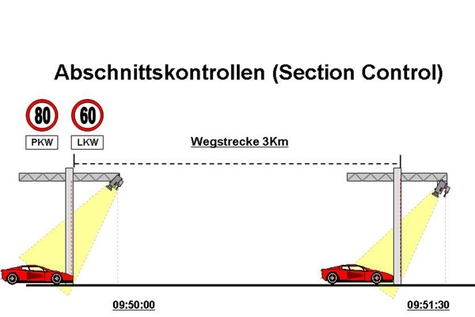
\includegraphics[scale=0.70]{pics/sc_functionality_basic.jpg}}
    \caption[Section Control Functionality]{\label{fig:Section Control Functionality}
	A basic Section Control system}
\end{figure}

%==========

\section{Problems}
\label{sec:1problems}

The main problem regarding these systems are privacy issues due to the fact that personal data is being stored before a violation of law occurs. 
This is the reason why people rightly raised objections against judgements made based on data gained from Section Control systems. 
\par According to Austria's "data privacy law" (DSG 2000) the storage of personal data is only permitted after committing an infringement. 
Now it gets quite obvious why these objections are justified and sustained. As a result an enactment from 
the Federal Ministry for Transport, Innovation and Technology is required \textit{per} system installed.
\par The current situation is quite unsatisfying hence improved ways of processing personal data are required to further improve 
data privacy and the installation of new systems.

%==========

\section{Objective}
\label{sec:1objective}

Austrian based company Kapsch TrafficCom wanted a prototype for a software which handles recording and storing of personal data
retrieved from an OCR camera on freeways. With the assistance of cryptographic algorithms the recorded data is fully encrypted and impervious to abuse 
during a vehicle's travel to the section's exit. This procedure requires just a software update on current systems without 
the need of any exchange of hardware. Existing systems become compliant with Austria's law at very low costs on the one hand and 
a great increase in privacy on the other hand. 

% --------------------------------------------------------------------------

\chapter{Software Design}
\section{UML}
\label{sec:2uml}

UML or Unified Modeling Language is a modeling language in the field of software design and engineering. 
It includes rules, graphical notations and introduces important terms to the user to simplify collaboration during
an entire software developing project. It was used during the development process and especially in the beginning
to get a better understanding which objects exist, what their properties are and how they interact with each other.

%==========

\section{Class Diagrams}
\label{sec:2classdiagrams}

The basic idea was a modular design due to the utilization of object-oriented programming language C++.
In the beginning a list of involved objects was created and the properties needed were figured out. The result
was converted into standardized UML class diagrams and formed the groundwork for the C++ implementation.

\paragraph{Note:} Items marked with "+" specify \textit{public elements} that can be accessed  from both inside and outside
the class, whereas "\#" marked items (\textit{protected elements}) can only be accessed from within the class or sub-classes respectively.
Items tagged "-" define \textit{private elements} that are only accessible within the class they are defined in.
This schema is valid for variables as well as functions.

\begin{figure}[p]
    \centerline{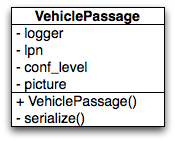
\includegraphics[scale=0.7]{pics/class_vehiclepassage.png}}
    \caption[Class VehiclePassage]{\label{fig:Class VehiclePassage}
	Class VehiclePassage representing a car}

	\begin{description}
	\item[lpn] the vehicles licence plate number
	\item[conf\_level] quality of optical character recognition (OCR)
	\item[picture] picture from OCR cam (not implemented)
	\end{description}
\end{figure}

\begin{figure}[p]
    \centerline{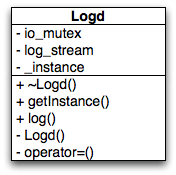
\includegraphics[scale=0.7]{pics/class_logd.png}}
    \caption[Class Logd]{\label{fig:Class Logd}
	Class Logd used for event logging purposes}
	
	\begin{description}
	\item[log()] used to write log entries to a file
	\end{description}
\end{figure}

\begin{figure}[p]
    \centerline{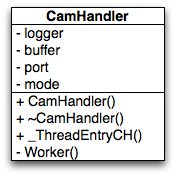
\includegraphics[scale=0.7]{pics/class_camhandler.png}}
    \caption[Class CamHandler]{\label{fig:Class CamHandler}
	Class CamHandler used to communicate with the OCR cameras}
	
	\begin{description}
	\item[Worker()] used to read data sent from on OCR cam
	\item[buffer] queue to enable asynchronous mode of operation
	\end{description}
\end{figure}

\begin{figure}[p]
    \centerline{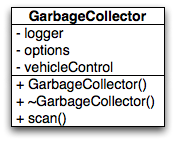
\includegraphics[scale=0.7]{pics/class_garbagecollector.png}}
    \caption[Class GarbageCollector]{\label{fig:Class GarbageCollector}
	Class GarbageCollector used to remove already exceeded vehicles}
	
	\begin{description}
	\item[vehicleControl] to get the list of vehicles
	\item[scan()] reads the list of known vehicles and removes already exceeded ones
	(where \textit{now} greater than \textit{minTS})
	\end{description}
\end{figure}

\begin{figure}[p]
    \centerline{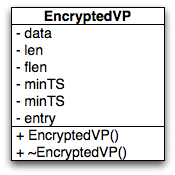
\includegraphics[scale=0.7]{pics/class_encryptedVP.png}}
    \caption[Class EncryptedVP]{\label{fig:Class EncryptedVP}
	Class EncryptedVP holds data of encrypted VehiclePassages}
	
	\begin{description}
	\item[data] encrypted data
	\item[len] data length
	\item[flen] fill length used for padding
	\item[entry] timestamp created when passing an OCR cam
	\item[minTS] calculated minimum time required to pass the monitored section
	\end{description}

    \centerline{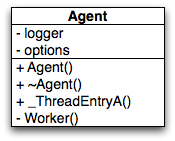
\includegraphics[scale=0.7]{pics/class_agent.png}}
    \caption[Class Agent]{\label{fig:Class Agent}
	Class Agent provides options for remote controlling the Section Control daemon}
\end{figure}

\begin{figure}[p]
    \centerline{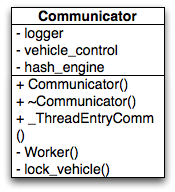
\includegraphics[scale=0.7]{pics/class_communicator.png}}
    \caption[Class Communicator]{\label{fig:Class Communicator}
	Class Communicator used to communicate with other Section Control daemons (e. g. entrance or exit)}
	
	\begin{description}
	\item[vehicle\_control] to get items from VehicleControl's list of vehicles
	\item[hash\_engine] to calculate hashes used to identify vehicles
	\item[lock\_vehicle] lock the vehicle so the gargabe collector cannot remove it accidentally
	\end{description}
\end{figure}

\begin{figure}[p]
    \centerline{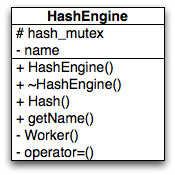
\includegraphics[scale=0.7]{pics/class_hashengine.png}}
    \caption[Class HashEngine]{\label{fig:Class HashEngine}
	Class HashEngine provides an abstract API for hash functions}
	
	\begin{description}
	\item[name] the name of the hash method (e.g. "MD5" or "SHA-1")
	\item[Hash()] returns the hash of the input data
	\end{description}

    \centerline{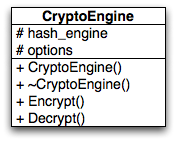
\includegraphics[scale=0.7]{pics/class_cryptoengine.png}}
    \caption[Class CryptoEngine]{\label{fig:Class CryptoEngine}
	Class CryptoEngine provides an abstract API for cryptographic functions}
	
	\begin{description}
	\item[name] the name of the cryptographic algorithm (e.g. "AES-256" or "DES")
	\item[Encrypt()] encrypts input data
	\item[Decrypt()] decrypts input data
	\end{description}
\end{figure}

\begin{figure}[p]
    \centerline{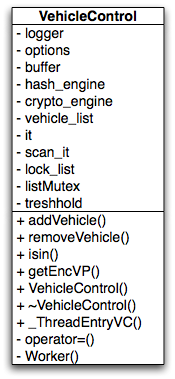
\includegraphics[scale=0.7]{pics/class_vehiclecontrol.png}}
    \caption[Class VehicleControl]{\label{fig:Class VehicleControl}
	Class VehicleControl managing stored vehicle data}
	
	\begin{description}
	\item[vehicle\_list] list containing all stored vehicles
	\item[treshhold] minimum OCR quality required
	\item[hash\_engine] access to hash functions
	\item[crypto\_engine] access to cryptographic functions
	\item[getEncVP()] get an encrypted VehiclePassage from the list
	\end{description}
\end{figure}

\begin{figure}[p]
    \centerline{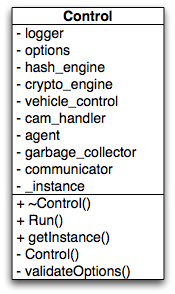
\includegraphics[scale=0.7]{pics/class_control.png}}
    \caption[Class Control]{\label{fig:Class Control}
	Class Control is used as a link between all components}
\end{figure}

%==========

\section{Used software}
\label{sec:2usedsw}

\begin{tabular} { l l l }
	\textbf{Windows}:	&	.NET Studio 2008		&	IDE								\\
	\textbf{Mac OS X}:	&	OmniGraffle				&	Diagramming software	\\
	\textbf{Linux}:			&	vim							&	Text editor 					\\
									&	GNU gcc					&	Compiler						\\
									&	GNU ld						&	Linker							\\
									&	Subversion				&	Revision control			\\
									&	Git							&	Revision control			\\
									&	tail							&	File display utility		\\
									&	netcat						&	OCR Cam simulation	\\
\end{tabular}

%==========

\section{Revision control}
\label{sec:2revcontrol}

When designing software it is always important to have a working history that keeps track of applied changes to the project.
In case of errors or misbehaving code it is very easy to compare (\textit{"to diff"}) the current code to previous versions (\textit{"revisions"})
and unveil the faulty code. 
\par During application development programmers add snap-shots to the revision control (\textit{"revisions"}) 
that can later be used to discard changes and revert to a working copy of the code. During the beginning of the project 
Subversion\footnote{\label{Apache:2} http://subversion.apache.org} was used to provide these services, 
but due to the lack of proper branching functionality git\footnote{\label{git:3} http://git-scm.com} was used henceforth.
\par Branching is used for parallel development where many people contribute to files under revision control.
The ability to branch offers a way to isolate changes to an independent tree without affecting the codebase. 
This feature is especially useful when the programmer wants to implement new experimental functionality which is normally done in the following way:

\begin{enumerate}
	\item Achieve a stable master branch
	\item Create a new branch and switch to that branch
	\item Write and commit the changes
	\item Change back to master branch
	\item Merge the changes
	\item Delete the testing / experimental branch
\end{enumerate}

Consider serious problems while adding new features in the testing branch. While the errors prevent the testing tree from working properly
the master branch is still fully functional and thus unaffected from changes made to the testing branch.
See~\ref{sec:appendix} for an example.

%==========

\section{Used libraries}
\label{sec:2libs}

Despite the fact that platform independence was not a required objective during the work on the Section Control daemon it
was tried to achieve this goal to keep the software as portable as possible. Changing the underlying infrastructure should
not affect the software. This is important when a company maintains various systems using different operating systems but 
still want to use the software without the need of serious changes.

\begin{itemize}
	\item \textbf{Boost C++ libraries} \hfill \\
		Boost provides portable C++ libraries which are either already included in the upcoming C++ standard (Technical report 1) or will be incorporated into the technical report 2.
		They offer another abstraction layer for operating system specific functions like threading, networking (ASIO), date and time functions, file system manipulation, program options 			and data serialization. Further details will be given in later chapters.
	\item \textbf{PolarSSL cryptographic C library} \hfill \\
		The PolarSSL libraries offer a simple API to the cryptographic and hash functions used in the Section Control daemon. Implementing cryptographic algorithms like AES is very 					sensitive, error-prone and it takes a long time to test and verify the code. To not reinvent the wheel the cryptographic library was used for AES encryption, MD5 as well as SHA-256 			hashing.
\end{itemize}

	
% --------------------------------------------------------------------------

\chapter{Implementation}
\section{Module Design}
\label{sec:3moddesign}

\begin{lstlisting}[label=The Singleton pattern,caption=The Singleton pattern]
	static Logd* getInstance() {
		if( !_instance )
        	_instance = new Logd();
		return _instance;
	}
\end{lstlisting}



%==========

\section{Functional interaction}
\label{sec:3interaction}
\section{Caveats}
\label{sec:3caveats}

% --------------------------------------------------------------------------

\chapter{Software tests}

% --------------------------------------------------------------------------

\chapter{Conclusion}




% Start labeling chapters with letters and calling them appendices
\appendix

 % Make the bibliography.
% \cleardoublepage
 %\phantomsection \addcontentsline{toc}{chapter}{Bibliography}
 %\begin{thebibliography}{00}
% \bibitem{Jackson1998}
%   J.~D. Jackson, {\em Classical Electrodynamics}, 3rd ed. (Wiley, New
%    York, 1998), \ p.\ 23.
% \bibitem{Peatross2000}
%    J.~Peatross, S.~A. Glasgow, and M.~Ware, ``Average energy flow of
%    optical pulses dispersive media,'' Phys.~Rev.~Lett. {\bf 84,} 2370--2373 (2000).
% \bibitem{intel}
  % notice the \url function that helps text wrapping in the \href
%    K. David, ``Intel's EUV lithography process line,''
%    \href{http://www.intel.com/technology/silicon/lithography.htm}
%    {\url{http://www.intel.com/technology/silicon/lithography.htm}}
%    (Accessed April 15, 2006).
%\end{thebibliography}

\chapter{Appendix}
\label{sec:appendix}

\begin{lstlisting}[label=Git revision control,caption=Git revision control]	
	\$ git status
	# On branch master
	nothing to commit (working directory clean)
	\$ git branch experimental
	$ git checkout experimental 
	Switched to branch 'experimental'
	$ edit files ...
	git commit -a
	[experimental f4e4220] edit main
 	1 files changed, 7 insertions(+), 0 deletions(-)
	$ git checkout master
	Switched to branch 'master'
	$ git merge experimental
	Updating ed66c24..f4e4220
	Fast-forward
	main.c |    7 +++++++
 	1 files changed, 7 insertions(+), 0 deletions(-)
	$ git branch -d experimental 
	Deleted branch experimental (was f4e4220).
\end{lstlisting}


 % Make the index
 \cleardoublepage
 \singlespace
 % NOTE: '\phantomsection' helps get the pdf bookmark to work right. You need
 % to put it before every manual addition to the table of contents
 \phantomsection
 \addcontentsline{toc}{chapter}{Index}
 \printindex

\end{document}
